\chapter{Latex Pointers}

TODO remove.

This chapter contains some examples on the usage of latex. Do not include in your final report.

\section{Figures}
From time to time, it's necessary to add pictures to your documents. Using LaTeX all pictures will be indexed automatically and tagged with successive numbers when using the figure environment and the graphicx package. We can reference the figure below using its label like this: Fig. \ref{fig:test_plot}.
\begin{figure}[H]
  \centering
  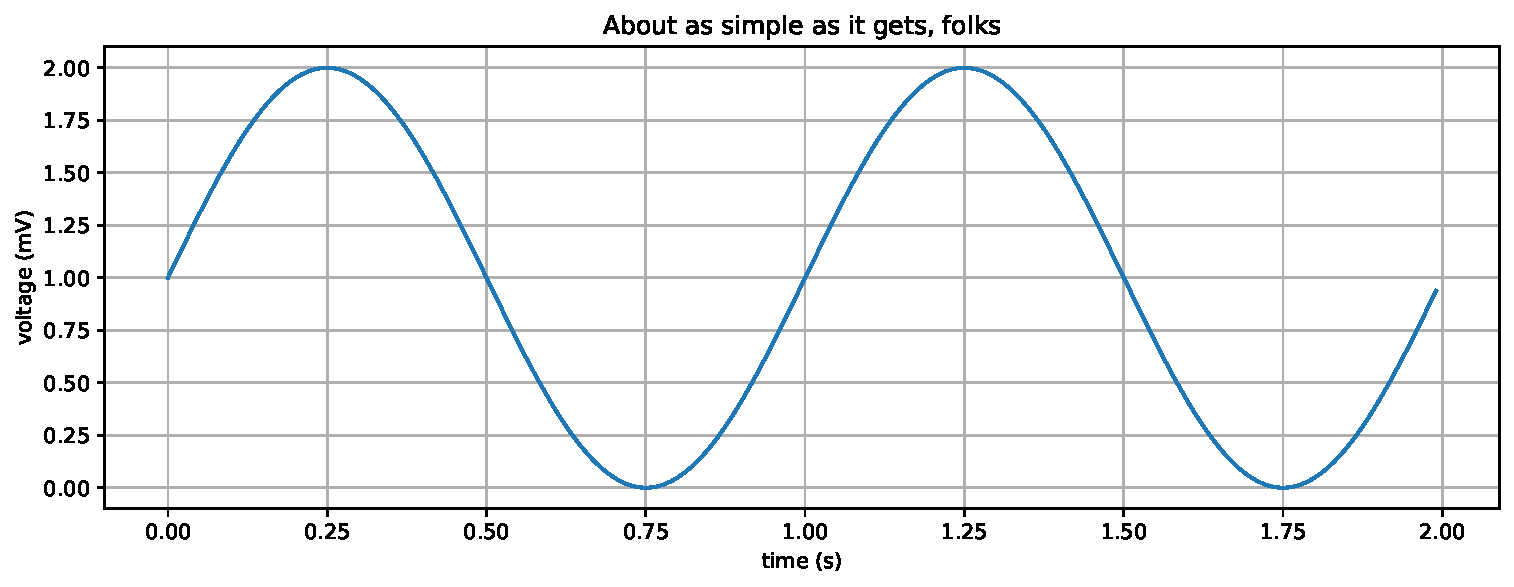
\includegraphics[width=0.8\linewidth]{./assets/images/test-plot.pdf}
  \caption{A sample graph}
  \label{fig:test_plot}
\end{figure}

Lots more information in this \href{https://www.latex-tutorial.com/tutorials/figures/}{tutorial}.


\section{Code Listing}
You can list code using the \emph{listings} package:

\begin{lstlisting}[language=Python,caption=Borg Pattern]
class Borg(object):
    __shared_state = {}

    def __init__(self):
        self.__dict__ = self.__shared_state
        self.state = 'Init'

    def __str__(self):
        return self.state
\end{lstlisting}

Lots more examples \href{https://www.overleaf.com/learn/latex/Code_listing}{here}.

\section{Math}
Here \ref{eq:limit} is an example of including an equation
\begin{equation}
  \lim_{x\to\infty} f(x)
  \label{eq:limit}
\end{equation}

More examples \href{https://www.latex-tutorial.com/tutorials/amsmath/}{here} and \href{https://www.overleaf.com/learn/latex/Mathematical_expressions}{here}.



\section{References}
Look up the bibtex references on google scholar or import from Mendeley or other reference managers. Add the bibtex snippet to the \emph{references.bib} file. Then cite the reference like this:

As explained in \cite{knuth2014art}, we also find that...

Lots more details \href{https://www.latex-tutorial.com/tutorials/bibtex/}{here}.
